%% =====================================================================
%%  TransKAN — SIBGRAPI 2026 poster
%%  Layout modelled on the HenriquesLab poster template (a0poster, 3 cols)
%%  Build: make   (pdfLaTeX)
%% =====================================================================
\documentclass[a0,portrait]{a0poster}

\usepackage[utf8]{inputenc}
\usepackage[T1]{fontenc}
\usepackage{times}
\usepackage[svgnames,table]{xcolor}
\usepackage{graphicx}
\usepackage{multicol}
\usepackage{booktabs}
\usepackage{amsmath,amssymb}
\usepackage[font=small,labelfont=bf,justification=justified,singlelinecheck=false]{caption}
\usepackage{fontawesome}
\usepackage{qrcode}
\usepackage{enumitem}
\usepackage{etoolbox}
\usepackage{tikz}
\usetikzlibrary{arrows.meta,positioning,calc,shapes.geometric,decorations.pathreplacing}
\usepackage{pgfplots}
\pgfplotsset{compat=1.18}

% ---------------------------------------------------------------------
%  Switches you may want to flip
% ---------------------------------------------------------------------
% Results bar chart metric: F1 (default) or AUC.
% F1 is the default because baseline AUCs in Table I equal their macro
% recall (i.e. they appear to be computed from hard labels), while the
% TransKAN AUC comes from softmax probabilities. Switch to AUC only once
% baseline AUCs are recomputed from probabilities.
\newif\ifchartauc \chartaucfalse
\newcommand{\chartlabel}{\ifchartauc macro AUC\else macro F1-score\fi}
\newcommand{\qrurl}{https://github.com/Silva015/tcc-2026}

% ---------------------------------------------------------------------
%  Colours
% ---------------------------------------------------------------------
\definecolor{kangreen}{RGB}{51,153,102}   % green used in the architecture figure
\definecolor{kangold}{RGB}{255,204,0}     % yellow used in the architecture figure
\definecolor{navyA}{RGB}{0,0,128}
\definecolor{navyB}{RGB}{58,86,170}
\definecolor{navyC}{RGB}{130,155,215}
\definecolor{navyD}{RGB}{200,212,238}
\definecolor{wound}{RGB}{160,30,40}
\definecolor{softgray}{RGB}{235,235,240}

% ---------------------------------------------------------------------
%  Layout helpers
% ---------------------------------------------------------------------
\setlength{\columnsep}{50pt}
\setlength{\columnseprule}{0pt}
\setlength{\parindent}{0pt}
\setlength{\parskip}{0.45em}
\captionsetup{skip=12pt}
\setlist{leftmargin=1.2em,itemsep=0.25em,topsep=0.3em}

\newcommand{\postersection}[1]{%
  \vspace{1.1em}%
  {\raggedright\color{NavyBlue}\LARGE\bfseries #1\par}%
  \vspace{0.15em}{\color{kangold}\rule{\linewidth}{5pt}}\par\vspace{0.4em}}

\newcommand{\figtitle}[1]{\textbf{#1}}

\tikzset{
  neuron/.style={circle,draw=black,line width=2pt,minimum size=1.3cm,inner sep=0pt,fill=white},
  chip/.style={rounded corners=8pt,draw=#1,line width=2pt,fill=#1!12,inner sep=10pt,align=center,font=\small},
  arrowline/.style={-{Latex[length=14pt,width=12pt]},line width=3pt},
}

\begin{document}

%% =====================================================================
%%  HEADER
%% =====================================================================
\begin{minipage}[t]{0.74\linewidth}
  \vspace{0pt}
  {\color{NavyBlue}\fontsize{62}{72}\selectfont\bfseries
   TransKAN: Transfer Learning and Kolmogorov--Arnold\\[0.1em]
   Networks for Gunshot Wound Classification\par}
  \vspace{1.0em}
  {\Large\bfseries Arthur Silva Carneiro \quad and \quad Pedro Garcia Freitas\par}
  \vspace{0.5em}
  {\large Department of Computer Science, University of Bras\'ilia (UnB), Bras\'ilia, Brazil\par}
  \vspace{0.3em}
  {\large \faEnvelope~arthur.carneiro@aluno.unb.br \quad \faEnvelope~pedro.freitas@unb.br
   \quad \faGithub~Silva015\par}
  \vspace{0.3em}
  {\normalsize\color{DimGray} SIBGRAPI 2026 \,---\, Conference on Graphics, Patterns and Images\par}
\end{minipage}%
\hfill
\begin{minipage}[t]{0.24\linewidth}
  \vspace{0pt}\raggedleft
  \IfFileExists{img/author.jpg}{%
    \includegraphics[height=11.5cm]{img/author.jpg}%
  }{%
    \tikz\node[draw=gray,line width=2pt,dashed,minimum width=9.5cm,minimum height=11.5cm,
               align=center,font=\small\color{gray}]{author photo\\(img/author.jpg)};%
  }\\[1.0em]
  \raisebox{-0.5\height}{
\includegraphics[height=5.2cm]{img/unb_logo.pdf}}\hspace{1.2cm}%
  \raisebox{-0.5\height}{\qrcode[height=5.5cm]{\qrurl}}
\end{minipage}

\vspace{1.2em}
{\color{NavyBlue}\rule{\linewidth}{6pt}}
\vspace{0.6em}

%% =====================================================================
%%  BODY
%% =====================================================================
\begin{multicols}{3}
\raggedcolumns

%% ------------------------------ COLUMN 1 ----------------------------
Telling an \textbf{entry} from an \textbf{exit} gunshot wound, and estimating
the \textbf{shooting distance}, are core forensic tasks. They still rely on
expert judgement and depend on lighting and imaging conditions at the scene.
Deep CNNs have been tried, but conventional fully connected (MLP) heads
struggle with the \emph{irregular, noisy and imbalanced} decision boundaries of
real forensic photographs.
\textbf{TransKAN} keeps a pre-trained \textbf{ResNet-152} backbone and replaces
its dense classifier with a \textbf{Kolmogorov--Arnold Network (KAN)} head,
which has \emph{learnable spline activations on every edge}.
It is validated on \textbf{GuWID}, a new database of
\textbf{2,551 real wound images} from Federal District Civil Police (PCDF)
casework.

\postersection{Real Forensic Evidence}

{\small\color{wound}\faExclamationTriangle~\textit{Contains real forensic imagery.}\par}
\vspace{0.3em}
\begin{center}
\resizebox{\linewidth}{!}{%
\begin{tikzpicture}[x=1cm,y=1cm]
  % raw photographs (same height)
  \node[anchor=north west,inner sep=0] (r1) at (0,0)     {\includegraphics[height=10cm]{img/wound_raw1.png}};
  \node[anchor=north west,inner sep=0] (r2) at (8.4,0)   {\includegraphics[height=10cm]{img/wound_raw2.png}};
  \node[anchor=north west,inner sep=0] (r3) at (17.4,0)  {\includegraphics[height=10cm]{img/wound_raw3.png}};
  % squared crops (same width)
  \node[anchor=north,inner sep=0,draw=kangold,line width=5pt] (c1) at ($(r1.south)+(0,-3.2)$) {\includegraphics[width=7.2cm]{img/wound_crop1.png}};
  \node[anchor=north,inner sep=0,draw=kangold,line width=5pt] (c2) at ($(r2.south)+(0,-3.2)$) {\includegraphics[width=7.2cm]{img/wound_crop2.png}};
  \node[anchor=north,inner sep=0,draw=kangold,line width=5pt] (c3) at ($(r3.south)+(0,-3.2)$) {\includegraphics[width=7.2cm]{img/wound_crop3.png}};
  \foreach \k in {1,2,3}{
    \draw[arrowline,NavyBlue] ($(r\k.south)+(0,-0.3)$) -- ($(c\k.north)+(0,0.4)$)
      node[midway,right,font=\large\bfseries,text=NavyBlue]{\faScissors};
  }
  \node[rotate=90,anchor=south,font=\large\bfseries,text=DimGray] at ($(r1.west)+(-0.2,0)$) {raw scene photo};
  \node[rotate=90,anchor=south,font=\large\bfseries,text=DimGray] at ($(c1.west)+(-0.9,0)$) {model input};
\end{tikzpicture}}
\captionof{figure}{\figtitle{From crime-scene photograph to model input.} Raw PCDF
photographs (top; note the forensic ruler) are cropped in GIMP to a square region
centred on the wound (bottom), then resized to $224\times224$. All three samples
are entry wounds.}
\end{center}

\postersection{GuWID: Gunshot Wound Image Database}

Built from records of \textbf{real homicide and suicide cases} examined by PCDF
forensic experts (UnB Research Ethics Committee, protocol
4418221.9.0000.0030). Labels (wound type, anatomical location, shooting distance)
were transcribed \emph{verbatim} from the forensic pathologist's autopsy
reports.

\begin{center}
\resizebox{\linewidth}{!}{%
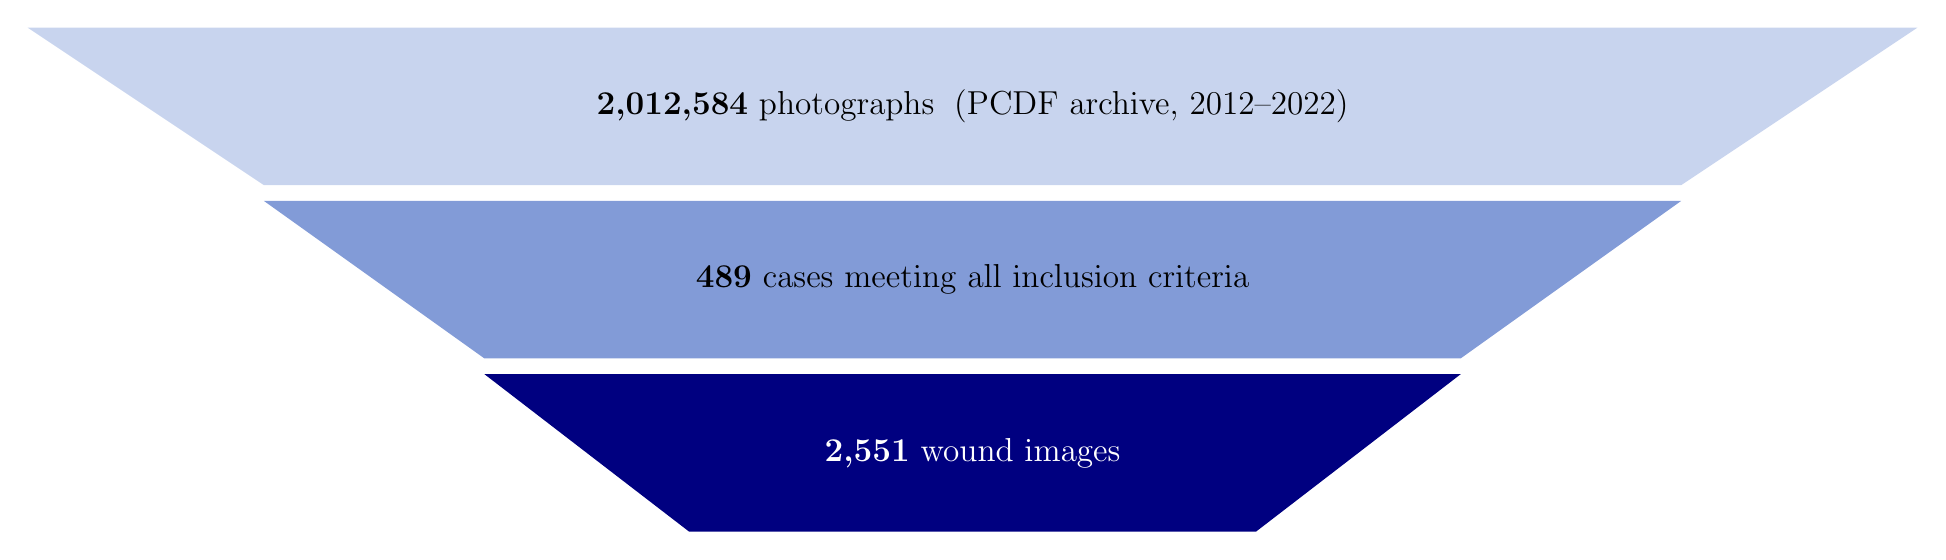
\begin{tikzpicture}[x=1cm,y=1cm,font=\large]
  \fill[navyD]  (0,6)   -- (24,6)   -- (21,4)   -- (3,4)   -- cycle;
  \fill[navyC]  (3,3.8) -- (21,3.8) -- (18.2,1.8)-- (5.8,1.8)-- cycle;
  \fill[NavyBlue](5.8,1.6)-- (18.2,1.6)-- (15.6,-0.4)-- (8.4,-0.4)-- cycle;
  \node[align=center] at (12,5)   {\textbf{2,012,584} photographs \;(PCDF archive, 2012--2022)};
  \node[align=center] at (12,2.8) {\textbf{489} cases meeting all inclusion criteria};
  \node[align=center,text=white] at (12,0.6) {\textbf{2,551} wound images};
\end{tikzpicture}}
\end{center}
\vspace{-0.4em}

% --- proportion strips -------------------------------------------------
\newlength{\stripw}\setlength{\stripw}{0.72\linewidth}
\newcommand{\seg}[6]{% x0, x1 (fractions), y, colour, inside label, text colour
  \fill[#4] ({#1*\stripw},#3) rectangle ({#2*\stripw},#3+1.6);
  \node[font=\small\bfseries,text=#6] at ({(#1+#2)/2*\stripw},#3+0.8) {#5};}
\begin{center}
\begin{tikzpicture}[x=1cm,y=1cm]
  % wound type
  \node[anchor=east,font=\small\bfseries,align=right] at (-0.3,6.8) {Wound\\type};
  \seg{0}{0.738}{6}{navyA}{Entry 1,883}{white}
  \seg{0.738}{1}{6}{wound}{Exit 668}{white}
  % MLSD (entry wounds)
  \node[anchor=east,font=\small\bfseries,align=right] at (-0.3,3.8) {Shooting\\distance};
  \seg{0}{0.8545}{3}{navyB}{Distant 1,609}{white}
  \seg{0.8545}{0.9777}{3}{navyC}{}{black}
  \seg{0.9777}{1}{3}{wound}{}{white}
  \draw[line width=1.5pt] ({0.916*\stripw},3) -- ({0.916*\stripw},2.3) node[below,font=\scriptsize]{Close 232};
  \draw[line width=1.5pt] ({0.989*\stripw},3) -- ({0.989*\stripw},1.5) node[below,font=\scriptsize]{Contact 42};
  % anatomical region
  \node[anchor=east,font=\small\bfseries,align=right] at (-0.3,-1.2) {Anatomical\\region};
  \seg{0}{0.5135}{-2}{navyA}{Trunk 1,310}{white}
  \seg{0.5135}{0.7283}{-2}{navyB}{\scriptsize Head/neck 548}{white}
  \seg{0.7283}{0.9255}{-2}{navyC}{\scriptsize Upper 503}{black}
  \seg{0.9255}{1}{-2}{navyD}{}{black}
  \draw[line width=1.5pt] ({0.963*\stripw},-2) -- ({0.963*\stripw},-2.7) node[below,font=\scriptsize]{Lower 190};
\end{tikzpicture}
\end{center}
\vspace{-0.6em}
\captionof{figure}{\figtitle{GuWID is heavily imbalanced}, reflecting the real
rarity of some injuries: exit wounds are 26\% of the data and contact shots
only 2.2\% of entry wounds. 95.5\% of images come from male victims, which
matches the regional profile of firearm deaths.}

%% ------------------------------ COLUMN 2 ----------------------------
\columnbreak

\postersection{TransKAN Architecture}

\begin{center}
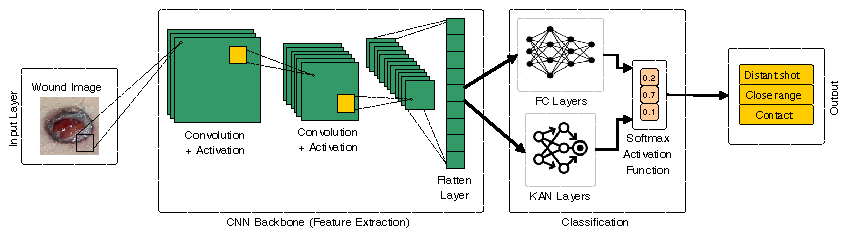
\includegraphics[width=\linewidth]{img/architecture.pdf}
\captionof{figure}{\figtitle{Pipeline.} A CNN backbone extracts features that
are flattened and passed to \emph{either} a conventional FC head (baseline)
\emph{or} our KAN head. The two heads are separate configurations, trained and
evaluated independently. They are drawn side by side only for comparison.}
\end{center}

\begin{center}
\resizebox{\linewidth}{!}{%
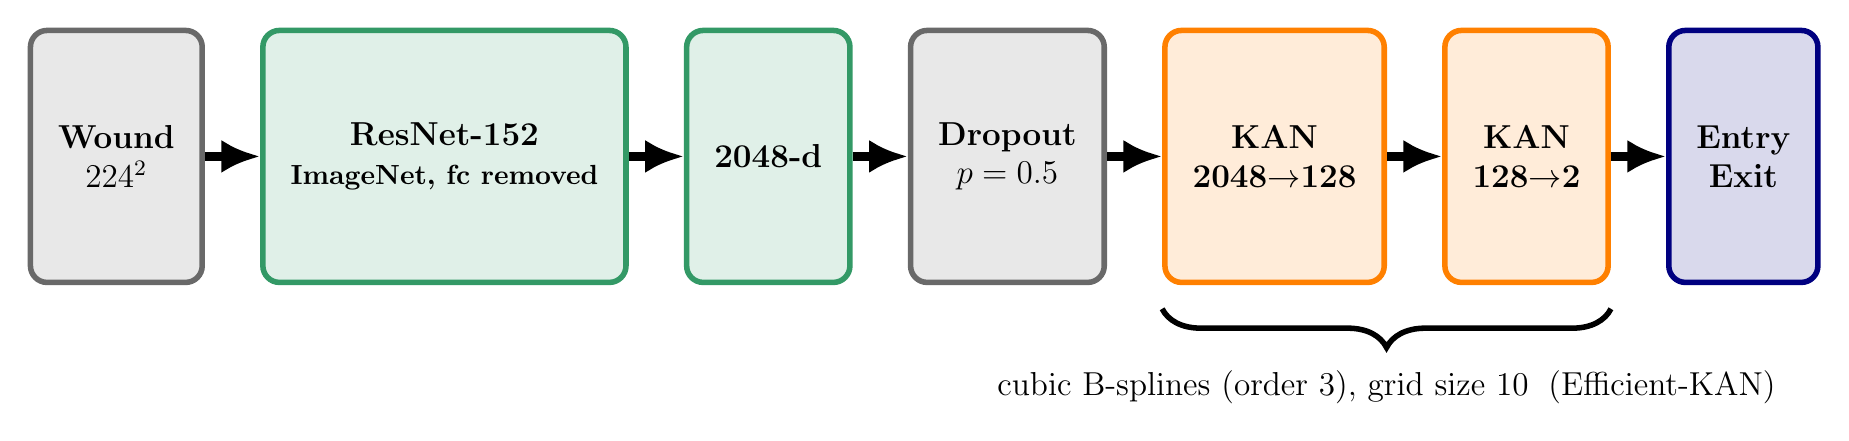
\begin{tikzpicture}[node distance=0.7cm,
    blk/.style={rounded corners=6pt,line width=2pt,draw=#1,fill=#1!15,minimum height=3.2cm,align=center,font=\large\bfseries,inner xsep=10pt}]
  \node[blk=DimGray]  (img) {Wound\\$224^2$};
  \node[blk=kangreen,right=of img] (bb) {ResNet-152\\{\normalsize ImageNet, fc removed}};
  \node[blk=kangreen,right=of bb]  (f)  {2048-d};
  \node[blk=DimGray,right=of f]    (d)  {Dropout\\$p=0.5$};
  \node[blk=orange,right=of d]     (k1) {KAN\\2048$\to$128};
  \node[blk=orange,right=of k1]    (k2) {KAN\\128$\to$2};
  \node[blk=NavyBlue,right=of k2]  (o)  {Entry\\Exit};
  \foreach \a/\b in {img/bb,bb/f,f/d,d/k1,k1/k2,k2/o} \draw[arrowline] (\a) -- (\b);
  \draw[decorate,decoration={brace,amplitude=14pt,mirror},line width=2pt]
     ($(k1.south west)+(0,-0.3)$) -- ($(k2.south east)+(0,-0.3)$)
     node[midway,below=18pt,font=\large]{cubic B-splines (order 3), grid size 10 \;(Efficient-KAN)};
\end{tikzpicture}}
\end{center}

\postersection{Why a KAN head? MLP vs.\ KAN}

\begin{center}
\resizebox{\linewidth}{!}{%
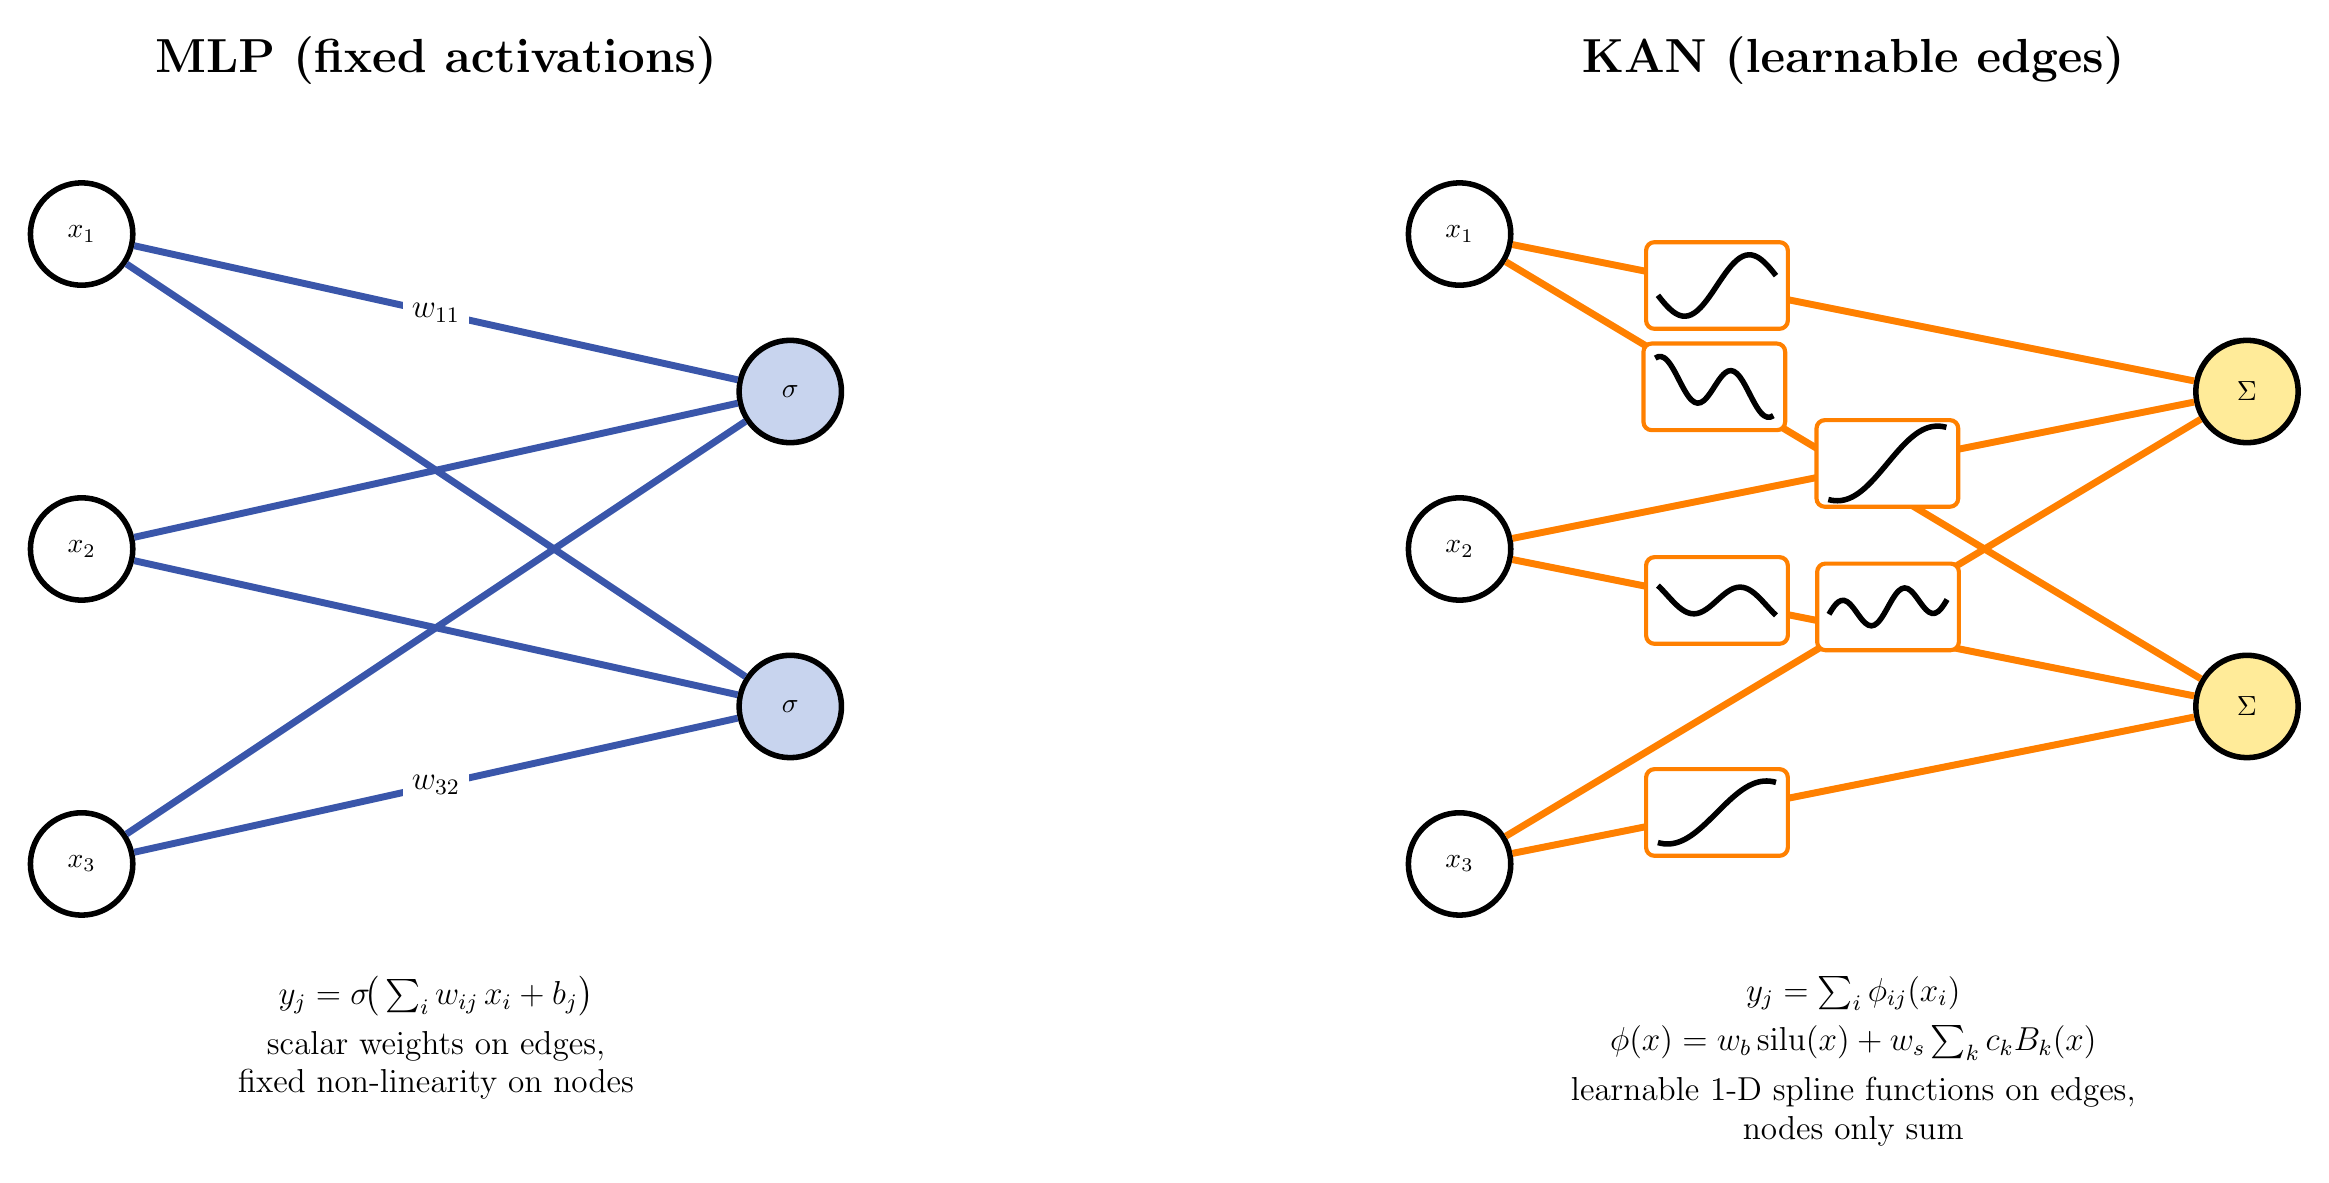
\begin{tikzpicture}[x=1cm,y=1cm]
  % ---------------- MLP ----------------
  \node[font=\LARGE\bfseries] at (4.5,10.2) {MLP (fixed activations)};
  \foreach \i/\y in {1/8,2/4,3/0} \node[neuron] (m\i) at (0,\y) {$x_{\i}$};
  \foreach \j/\y in {1/6,2/2} \node[neuron,fill=navyD] (mo\j) at (9,\y) {$\sigma$};
  \foreach \i in {1,2,3} \foreach \j in {1,2} \draw[line width=2.5pt,navyB] (m\i) -- (mo\j);
  \node[fill=white,font=\large] at ($(m1)!0.5!(mo1)$) {$w_{11}$};
  \node[fill=white,font=\large] at ($(m3)!0.5!(mo2)$) {$w_{32}$};
  \node[align=center,font=\large,anchor=north] at (4.5,-1.3) {$y_j=\sigma\!\big(\sum_i w_{ij}\,x_i + b_j\big)$\\[4pt]
     scalar weights on edges,\\ fixed non-linearity on nodes};
  % ---------------- KAN ----------------
  \begin{scope}[xshift=17.5cm]
  \node[font=\LARGE\bfseries] at (5,10.2) {KAN (learnable edges)};
  \foreach \i/\y in {1/8,2/4,3/0} \node[neuron] (k\i) at (0,\y) {$x_{\i}$};
  \foreach \j/\y in {1/6,2/2} \node[neuron,fill=kangold!40] (ko\j) at (10,\y) {$\Sigma$};
  \foreach \i in {1,2,3} \foreach \j in {1,2} \draw[line width=2.5pt,orange] (k\i) -- (ko\j);
  % small spline insets on every edge
  \foreach \i/\j/\a/\b/\c/\p in {1/1/4/0.35/0.1/0.3, 1/2/7/0.25/-0.2/0.3, 2/1/3/0.3/0.3/0.55,
                                2/2/5/0.2/-0.1/0.3, 3/1/8/0.2/0.2/0.55, 3/2/2.5/0.4/0.0/0.3}{
    \path (k\i) -- (ko\j) coordinate[pos=\p] (e\i\j);
    \begin{scope}[shift={(e\i\j)}]
      \draw[fill=white,draw=orange,line width=1.5pt,rounded corners=3pt] (-0.9,-0.55) rectangle (0.9,0.55);
      \draw[line width=2pt,black,domain=-0.75:0.75,samples=40,smooth]
            plot (\x,{\b*sin(deg(\a*\x))+\c*\x});
    \end{scope}}
  \node[align=center,font=\large,anchor=north] at (5,-1.3) {$y_j=\sum_i \phi_{ij}(x_i)$\\[4pt]
     $\phi(x)=w_b\,\mathrm{silu}(x)+w_s\sum_k c_k B_k(x)$\\[4pt]
     learnable 1-D spline functions on edges,\\ nodes only sum};
  \end{scope}
\end{tikzpicture}}
\end{center}
\captionof{figure}{\figtitle{Edges learn their own activation.} Each KAN edge
is a B-spline $\phi_{ij}$ whose shape is learned. This gives the classifier the
flexibility to fit irregular boundaries between morphologically similar wounds
\emph{without} extra depth, and only in the head, so the trainable parameter
count stays modest on a few thousand images. The design is motivated by the
Kolmogorov--Arnold representation theorem.}

\postersection{Imbalance Handling \& Augmentation}

\begin{center}
\resizebox{\linewidth}{!}{%
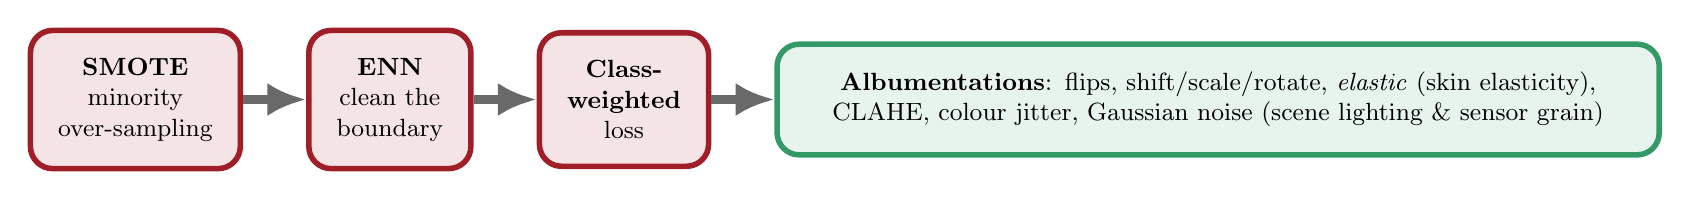
\begin{tikzpicture}[node distance=0.8cm]
  \node[chip=wound] (s) {\textbf{SMOTE}\\minority\\over-sampling};
  \node[chip=wound,right=of s] (e) {\textbf{ENN}\\clean the\\boundary};
  \node[chip=wound,right=of e] (w) {\textbf{Class-}\\\textbf{weighted}\\loss};
  \node[chip=kangreen,right=of w,text width=10.5cm] (a) {\textbf{Albumentations}: flips, shift/scale/rotate,
     \emph{elastic} (skin elasticity), CLAHE, colour jitter,
     Gaussian noise (scene lighting \& sensor grain)};
  \foreach \p/\q in {s/e,e/w,w/a} \draw[arrowline,DimGray] (\p) -- (\q);
\end{tikzpicture}}
\end{center}
\vspace{-0.3em}
{\small All steps are \textbf{re-fit inside each training fold only}, so
validation and test data are never touched.\par}

\postersection{Leakage-Free Evaluation}

\begin{center}
\resizebox{\linewidth}{!}{%
\begin{tikzpicture}[x=1cm,y=1cm]
  \foreach \f in {1,...,5}{
    \node[anchor=east,font=\large\bfseries] at (-0.3,-\f*1.5+0.6) {Fold \f};
    \foreach \b in {1,...,5}{
      \pgfmathsetmacro{\istest}{\b==\f ? 1 : 0}
      \ifdim\istest pt=1pt
        \fill[kangold,draw=black,line width=1.5pt] (\b*3.6-3.6,-\f*1.5) rectangle ++(3.4,1.2);
        \node[font=\normalsize\bfseries] at (\b*3.6-1.9,-\f*1.5+0.6) {test};
      \else
        \fill[navyC,draw=black,line width=1.5pt] (\b*3.6-3.6,-\f*1.5) rectangle ++(3.4,1.2);
        \node[font=\normalsize,text=white] at (\b*3.6-1.9,-\f*1.5+0.6) {train};
      \fi}}
  % a "case" with several photos, all falling in the same fold
  \node[font=\large,align=left,anchor=west] at (18.6,-3.9) {\faUser~case \#17\\
      {\color{wound}\faCamera\,\faCamera\,\faCamera} 3 photos\\ $\Rightarrow$ one fold only};
  \draw[arrowline,wound] (18.4,-3.9) -- (15.9,-4.5);
\end{tikzpicture}}
\end{center}
\vspace{-0.3em}
{\small One victim may have several photographs of the \emph{same} wound.
We use \textbf{grouped, stratified 5-fold cross-validation by case ID}, so no
wound appears in both training and test data. \textbf{All 12 baseline families were
re-trained under exactly the same protocol}, and out-of-fold predictions are
aggregated into the final metrics.\par}

\postersection{Take-home Messages}
\begin{itemize}
  \item[\color{kangreen}\faCheckCircle] Replacing only the \textbf{classifier head}
        (MLP$\to$KAN) on a ResNet-152 improves precision, F1 and class
        separation (AUC) on real forensic images.
  \item[\color{kangreen}\faCheckCircle] \textbf{GuWID}: 2,551 authentic wound images,
        labelled from autopsy reports.
  \item[\color{kangreen}\faCheckCircle] \textbf{Case-grouped} cross-validation
        removes the photo-level leakage that inflates results.
\end{itemize}

%% ------------------------------ COLUMN 3 ----------------------------
\columnbreak

\postersection{Two-Phase Training}

\begin{center}
\resizebox{\linewidth}{!}{%
\begin{tikzpicture}[x=0.4cm,y=1cm]
  \fill[DimGray!35]  (0,0) rectangle (15,1.4);
  \fill[kangreen!70] (15,0) rectangle (60,1.4);
  \node[font=\large\bfseries] at (7.5,0.7) {\faLock~Phase 1};
  \node[font=\large\bfseries,text=white] at (37.5,0.7) {\faUnlock~Phase 2: full fine-tuning};
  \foreach \e in {1,15,60} \node[below,font=\normalsize] at (\e,0) {\e};
  \node[below,font=\normalsize\itshape] at (22,0) {epoch};
  \node[align=left,anchor=north west,font=\normalsize] at (0,-1.1)
     {backbone frozen, head only\\AdamW, lr $10^{-3}$, wd $10^{-2}$};
  \node[align=left,anchor=north west,font=\normalsize] at (32,-1.1)
     {all layers, lr $10^{-5}$,\\CosineAnnealingLR};
  \draw[line width=2.5pt,NavyBlue,domain=16:60,samples=60,smooth]
     plot (\x,{2.2+0.7*cos(180*(\x-16)/44)}) ;
  \node[font=\small,text=NavyBlue,anchor=south west] at (17,2.9) {cosine lr decay};
\end{tikzpicture}}
\end{center}

\postersection{Results: Entry vs.\ Exit}

% --- big number tiles --------------------------------------------------
\newcommand{\tile}[3]{%
  \begin{tikzpicture}
    \node[rounded corners=10pt,fill=softgray,minimum width=0.225\linewidth,minimum height=5.8cm,
          align=center] {{\small\bfseries #1}\\[4pt]{\color{kangreen}\fontsize{58}{60}\selectfont\bfseries #2}\\[6pt]
          {\small\color{DimGray}ResNet-152: #3}};
  \end{tikzpicture}}
\begin{center}
\tile{macro F1}{0.832}{0.824}\hfill\tile{macro Precision}{0.847}{0.827}\hfill
\tile{Accuracy}{0.871}{0.869}\hfill\tile{macro AUC}{0.893}{0.821}
\end{center}

\begin{center}
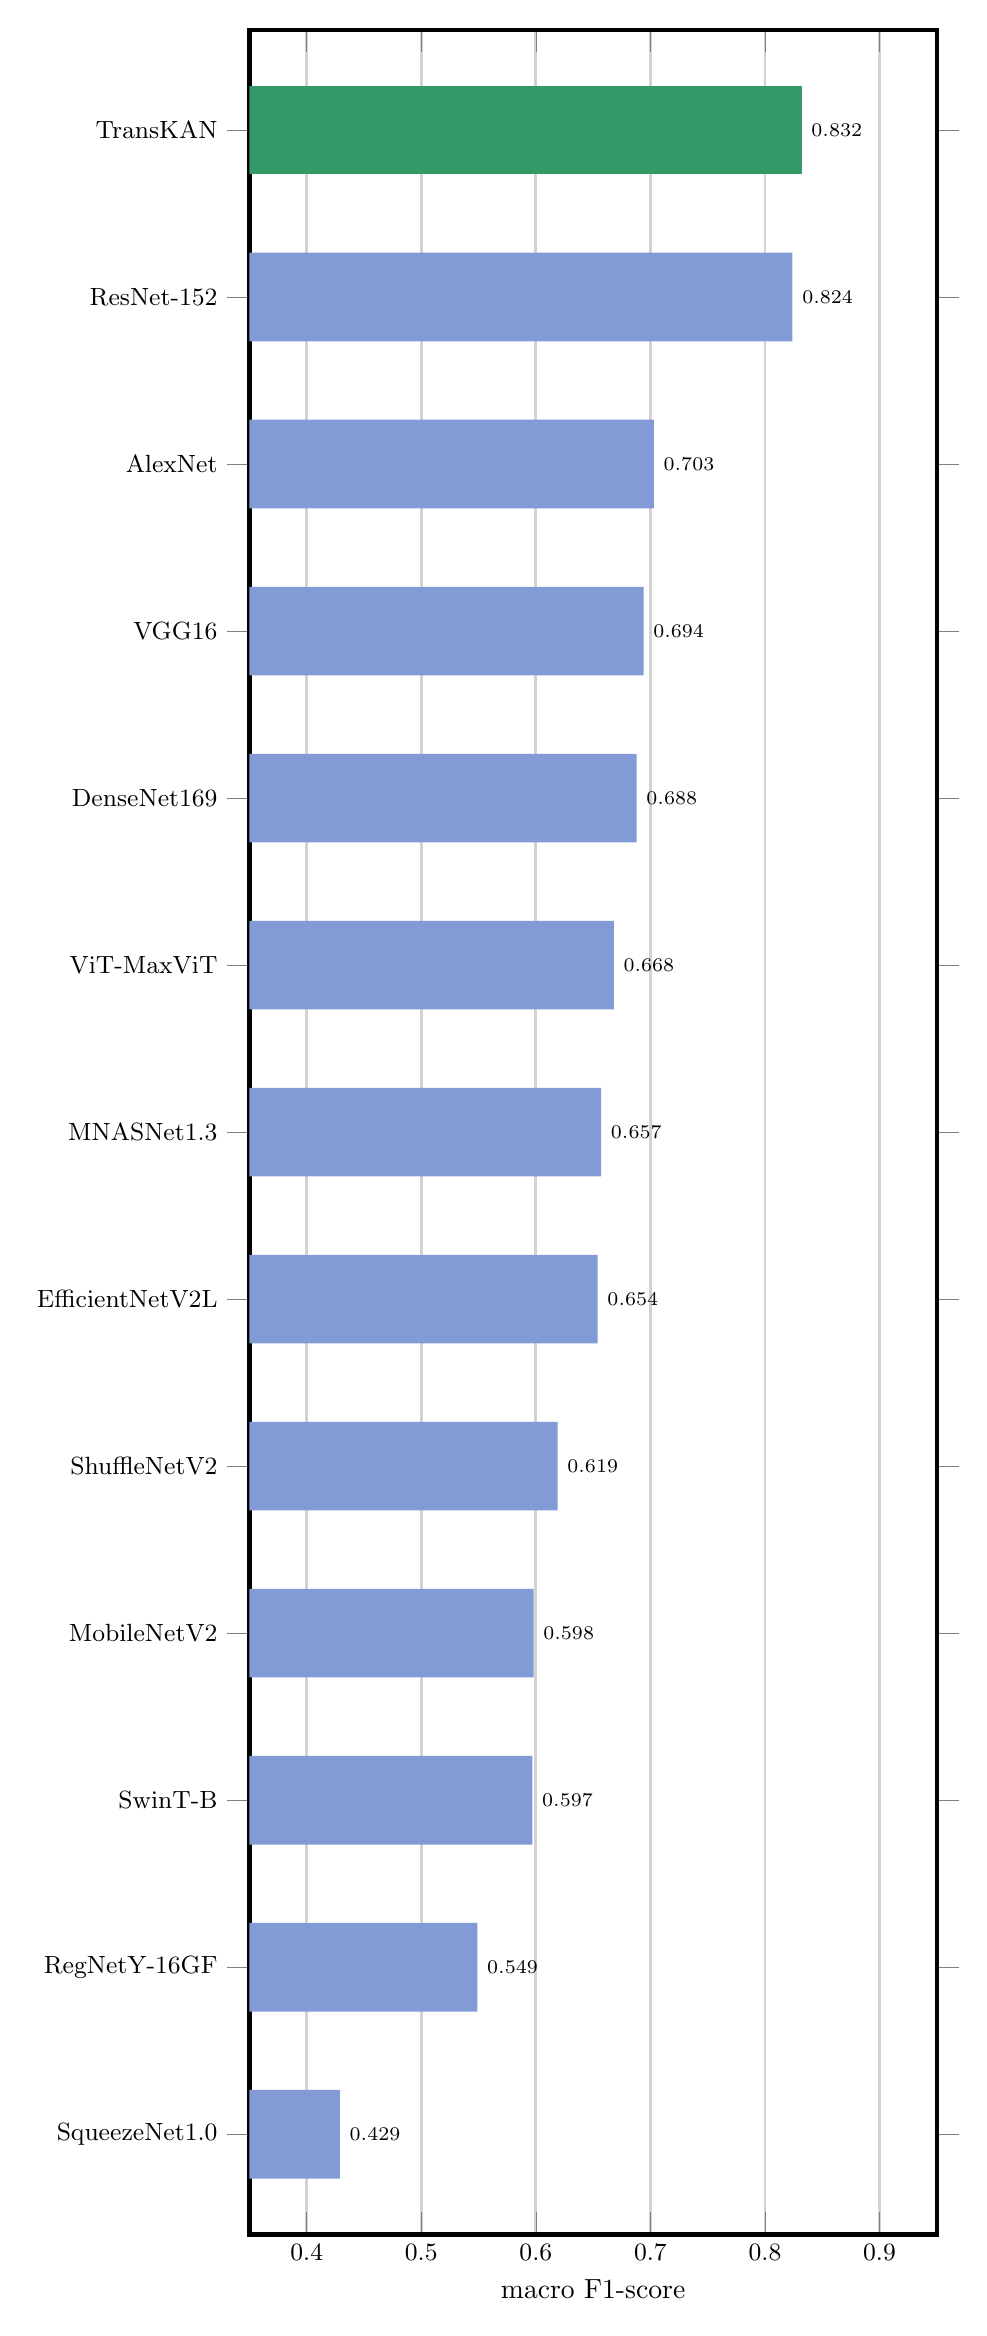
\begin{tikzpicture}
\begin{axis}[
    xbar, bar width=32pt, scale only axis, width=0.72\linewidth, height=28cm,
    y dir=reverse, ytick={TransKAN,ResNet-152,AlexNet,VGG16,DenseNet169,ViT-MaxViT,MNASNet1.3,EfficientNetV2L,ShuffleNetV2,MobileNetV2,SwinT-B,RegNetY-16GF,SqueezeNet1.0}, yticklabel style={font=\small}, yticklabel={\ifdefstring{\tick}{TransKAN}{\textbf{\color{kangreen}TransKAN}}{\tick}},
    symbolic y coords={TransKAN,ResNet-152,AlexNet,VGG16,DenseNet169,ViT-MaxViT,MNASNet1.3,EfficientNetV2L,ShuffleNetV2,MobileNetV2,SwinT-B,RegNetY-16GF,SqueezeNet1.0},
    xmin=0.35, xmax=0.95, xtick={0.4,0.5,0.6,0.7,0.8,0.9},
    xticklabel style={font=\small,/pgf/number format/fixed,/pgf/number format/precision=1},
    xlabel={\chartlabel},
    xlabel style={font=\normalsize},
    nodes near coords, nodes near coords align={horizontal},
    every node near coord/.append style={font=\scriptsize,/pgf/number format/fixed,/pgf/number format/precision=3,/pgf/number format/zerofill},
    axis line style={line width=1.5pt}, major tick length=8pt, enlarge y limits=0.05,
    xmajorgrids, grid style={DimGray!30,line width=1pt},
  ]
  \ifchartauc
  \addplot[fill=navyC,draw=none,bar shift=0pt] coordinates {
     (0.821,ResNet-152) (0.716,AlexNet) (0.685,VGG16) (0.679,DenseNet169) (0.653,ViT-MaxViT)
     (0.656,MNASNet1.3) (0.638,EfficientNetV2L) (0.614,ShuffleNetV2) (0.593,MobileNetV2)
     (0.591,SwinT-B) (0.549,RegNetY-16GF) (0.500,SqueezeNet1.0)};
  \addplot[fill=kangreen,draw=none,bar shift=0pt] coordinates {(0.893,TransKAN)};
  \else
  \addplot[fill=navyC,draw=none,bar shift=0pt] coordinates {
     (0.824,ResNet-152) (0.703,AlexNet) (0.694,VGG16) (0.688,DenseNet169) (0.668,ViT-MaxViT)
     (0.657,MNASNet1.3) (0.654,EfficientNetV2L) (0.619,ShuffleNetV2) (0.598,MobileNetV2)
     (0.597,SwinT-B) (0.549,RegNetY-16GF) (0.429,SqueezeNet1.0)};
  \addplot[fill=kangreen,draw=none,bar shift=0pt] coordinates {(0.832,TransKAN)};
  \fi
\end{axis}
\end{tikzpicture}
\captionof{figure}{\figtitle{Wound-type classification, grouped 5-fold CV.} Best
variant of each architecture family. Lightweight models (MobileNet, ShuffleNet,
SqueezeNet) form the lower bound. Isotropic ViTs are inconsistent at this data
scale. Deep residual backbones are strongest, and \textbf{TransKAN matches or
exceeds ResNet-152 on every primary metric}.}
\end{center}


\vspace{0.4em}
\begin{center}
{\small
\begin{tabular}{l*{5}{c}}
\toprule
 & Precision & Recall & F1 & AUC & Specificity\\
 & \scriptsize macro / micro & \scriptsize macro / micro & \scriptsize macro / micro & \scriptsize macro / micro & \scriptsize macro / micro\\
\midrule
ResNet-152 & .827 / .869 & .821 / .869 & .824 / .869 & .821 / .821 & .821 / .869\\
\rowcolor{kangreen!15}\textbf{TransKAN} & \textbf{.847} / \textbf{.871} & .821 / \textbf{.871} & \textbf{.832} / \textbf{.871} & \textbf{.893} / \textbf{.924} & .821 / \textbf{.871}\\
\bottomrule
\end{tabular}}
\captionof{table}{\figtitle{Head-to-head with the strongest baseline} (out-of-fold,
grouped 5-fold CV). In this binary task, the micro averages equal accuracy.}
\end{center}

\postersection{Future Work}
Joint multi-task entry/exit and MLSD (contact / close-range / distant)
estimation. Wavelet-based KANs to cut cost. External validation on
international forensic databases. Code and data will be released after
acceptance.

\vspace{0.6em}
{\footnotesize
\textbf{References.}
[1]~Z.~Liu \emph{et al.}, ``KAN: Kolmogorov--Arnold Networks,'' ICLR 2025.
[2]~R.~Queiroz Nogueira Lira \emph{et al.}, ``Deep learning-based human gunshot
wounds classification,'' \emph{Int.\ J.\ Legal Med.}, 139(2), 2025.
[3]~K.~He \emph{et al.}, ``Deep residual learning for image recognition,'' CVPR 2016.
[4]~Efficient-KAN, github.com/Blealtan/efficient-kan.
[5]~A.~Buslaev \emph{et al.}, ``Albumentations,'' \emph{Information}, 11(2), 2020.
\par\vspace{0.4em}
\textbf{Acknowledgements.} We thank the forensic experts of the Federal District
Civil Police (PCDF) for the case records and annotations.\par}

\end{multicols}
\end{document}
